\begin{itemize}
    \item Beschreibt die Grundüberlegungen der realisierten Lösung (Konstruktion/Entwurf) und die Realisierung als Simulation, als Prototyp oder als Software-Komponente etc.
    \item Hier beschreiben Sie Ihre gemachte Arbeit. Dazu braucht es eine Beschreibung des Vorgehens, aller Arbeitsschritte usw.
    \item (Definiert Messgrössen, beschreibt Mess- oder Versuchsaufbau, beschreibt und dokumentiert Durchführung der Messungen/Versuche)
    \item Bildmaterial erleichtert das Verständnis.
    \item (Experimente)
    \item Immer mit Aufbau und Vorgehen; Bildmaterial erleichtert das Verständnis.
    \item (Lösungsweg)
    \item Inkl. theoretische Herleitung der Lösung
    \item (Modell)
    \item (Eingesetzte Software)
    \item Die Funktionen von verwendeten Computerprogrammen zu Simulationszwecken, Berechnungen etc. sollen beschrieben werden. Dies soll aber in Worten, Formeln und geeigneten Darstellungen (z.B. Fluss- diagrammen) geschehen. Allfälliger Programmcode ist in einem Anhang zu dokumentieren.
    \item (Tests und Validierung)
\end{itemize}

\textbf{Marco's Proposal}
\begin{itemize}
    \item Anfangs High Level Overview Mischung, Kapitel ersichtlich was kommt Flussdiagram (um dieses haben wir dann die Prozessmethoden)
    \item Vorgehensmethode => Kanban und Scrum, maybe V-Model?
    \item Setup technisch, lokale Linux VM, ROS Installation, VS Code als IDE, GitHub Repos, GitHub Actions CI/CD (maybe?), Deployment Architektur
    \item Overview Architektur ROS und Code, Grundüberlegung => Path Planning Package in ROS, Prototyp Architektur zeigen, Explo und Opt Algos, erhaltet Input und sendet Input
    \item Messages (interfaces und fszhaw msgs) (System aussen)
    \item Path Planner Node
    \item Exploration Algorithm
    \item Optimization Service Node
    \item Optimization Algorithm
    \item Verifikation und Validierungen (Code Reviews, Fehlerfälle: Cones gehen verloren, Cones andere Seite entdeckt, allg Fehlerannahmen)
    \item Testing mit Maps, Cone Publisher und Planned Trajectory Subscriber (mocks), utils wie track plotter, trackconfig
    \item Setup eher im Projektanhang: Weekly meetings, Review every other week, Mitarbeit mit anderen BA Teams in Driverless und gesamt Verein (Working Saturday, Hilfe im Workshop, Ausstellung Conecto ZHAW)
    \item In Resultate Kapitel, Vergleich erste Algorithmen und Versuche: erste Überlegungen und Tests, alter path planner zhaw, dann densify und interpolate, rrt max hamburg, komplexer algo à la ultimate und dann jetzige implementation, zuerst was hat eth mit mpcc, dann global racetrajectory von tumftm
\end{itemize}

This chapter describes which approaches and methods have been used to solve the problem to find algorithms which calculate the optimum path on a racetrack. The V-Model was used to plan the overall project as shown in figure \ref{fig:High Level Project Overview}. Scrum was used for the meetings that were held with the supervisors and the driverless team to accomplish the planning of the sprints. Further explanation on the planning process is described in the section \ref{sec:Planning Methods}. After the planning section the architecture design in section \ref{sec:Architecture Design} is explained. The algorithms are explained in section \ref{sec:Exploration Algorithm} for the exploration and section \ref{sec:Optimization Algorithm} for the optimization algorithm. Lastly the integration and verification process is described in section \ref{sec:Integration and Verification}.

\begin{figure}[H]
    \centering
    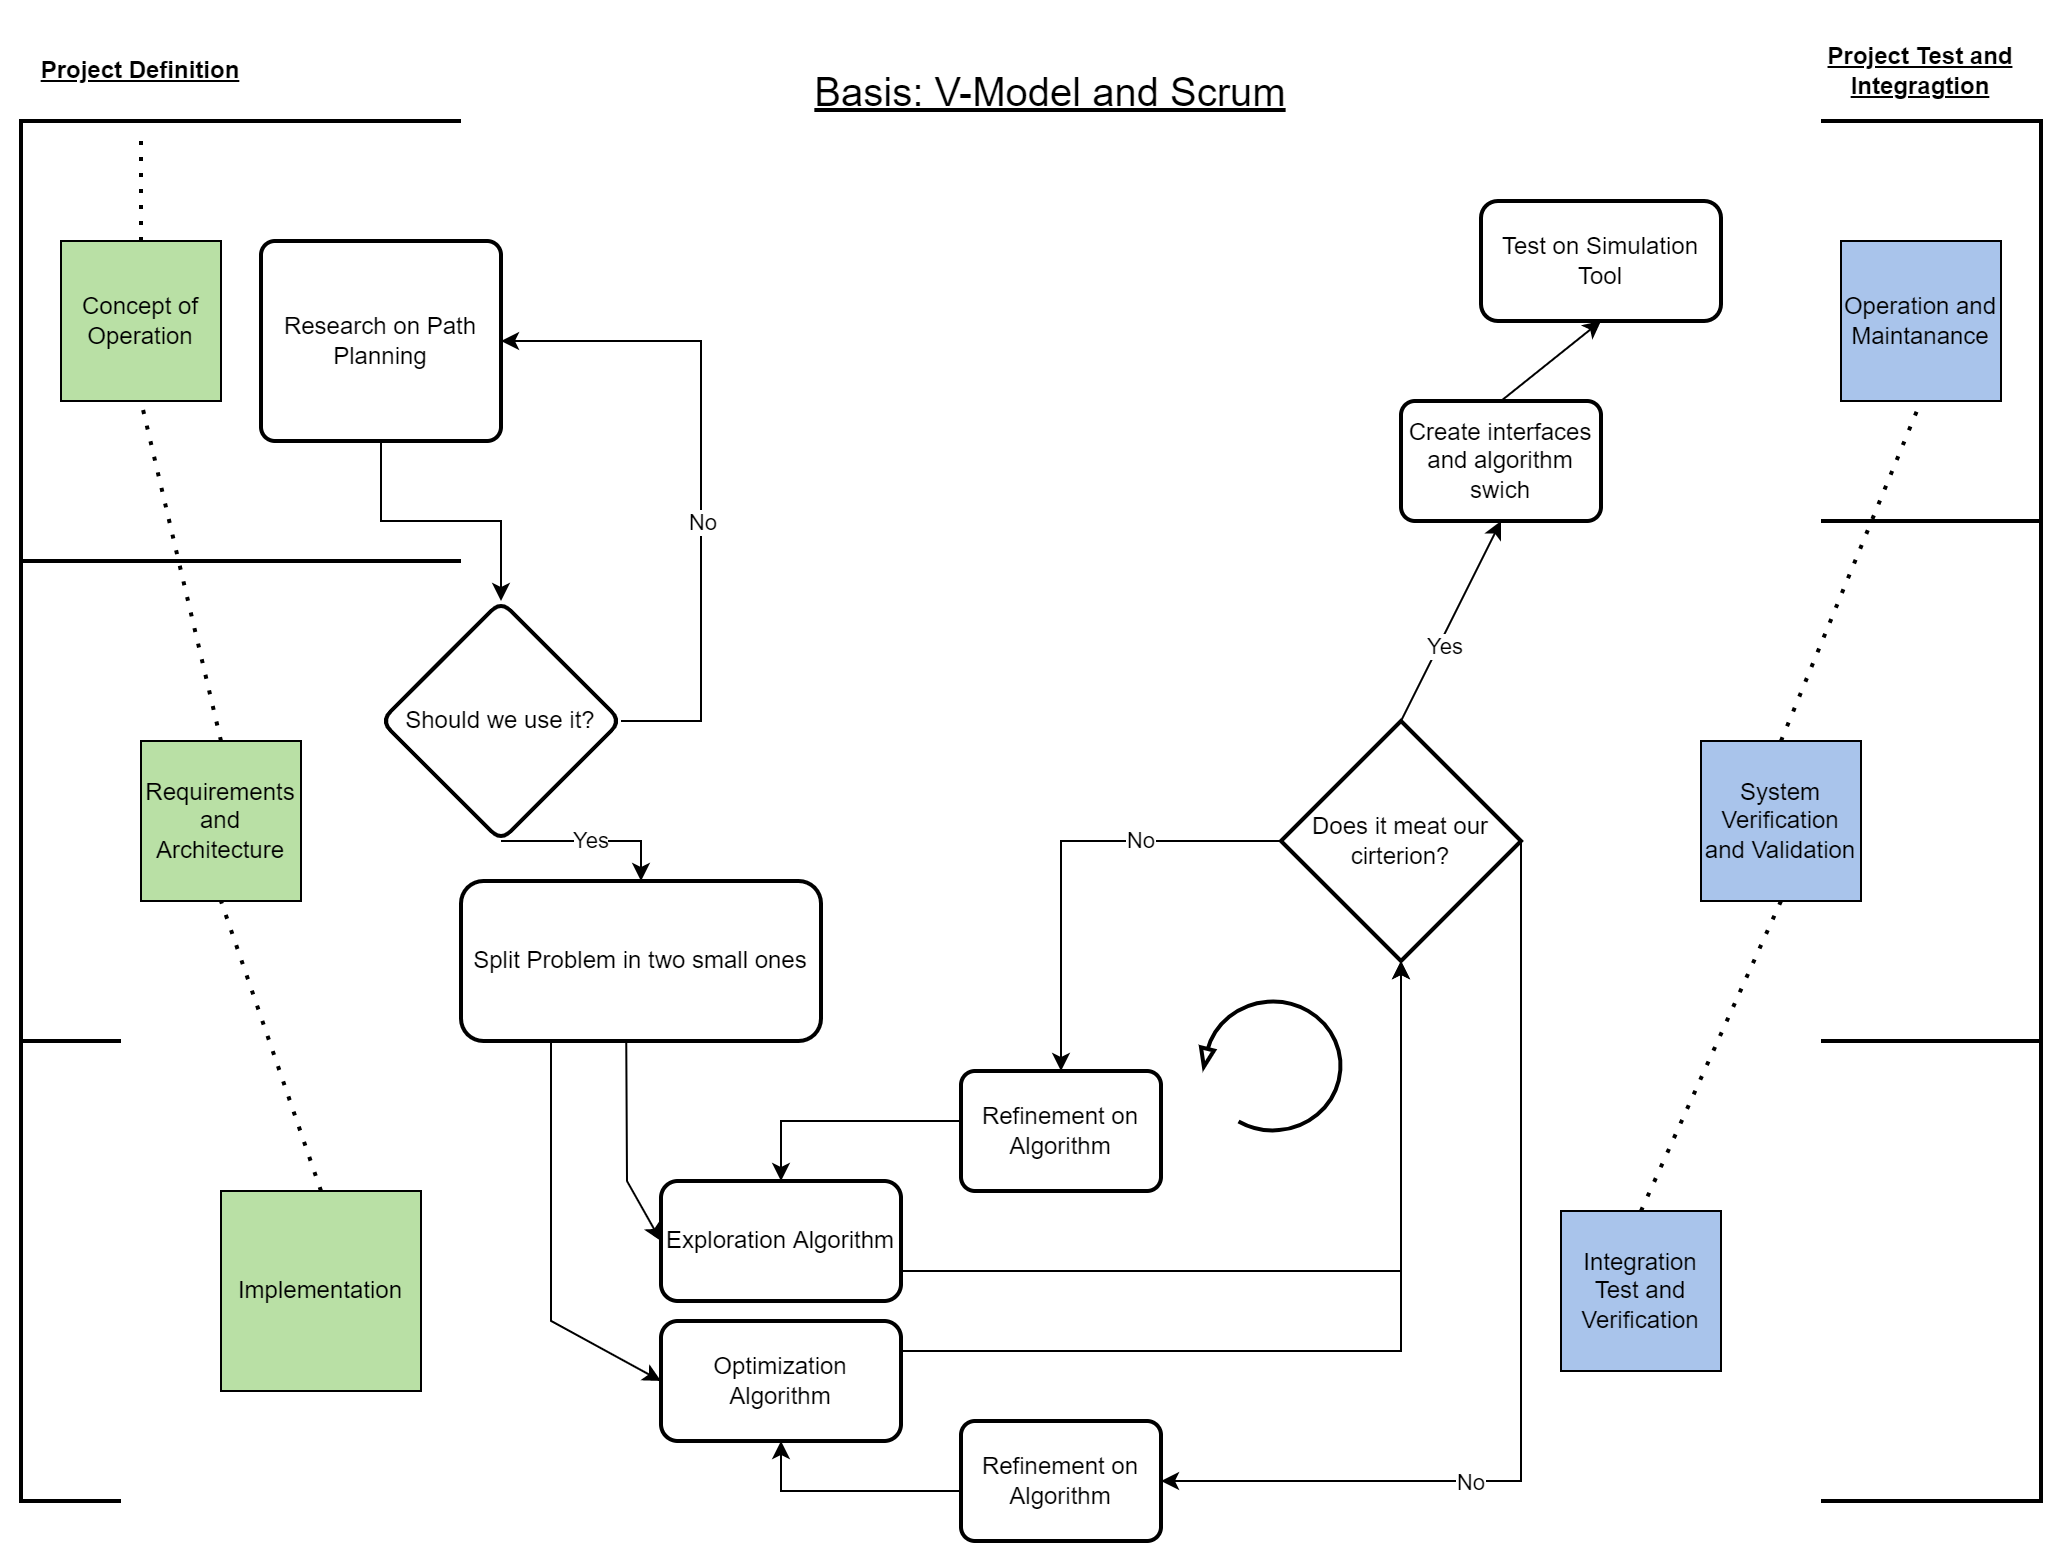
\includegraphics[width=\columnwidth]{High_Level_Project_Overview.png}
    \caption{The high level project overview gives an illustration which approaches and methods have been used to realize the project.}
    \label{fig:High Level Project Overview}
\end{figure}

\section{Planning Methods} \label{sec:Planning Methods}
To accomplish complex tasks in a team or alone there has to be a certain plan. In modern Software Engineering the method Scrum is very common as an agile planning method. As for an overall plan the V-Model was used.

\subsection{V-Model} \label{sec:Planning Method: V-Model}
The V-Model consists of several stages as shown in figure \ref{fig:V-Model}. 
\begin{figure}[H]
    \centering
    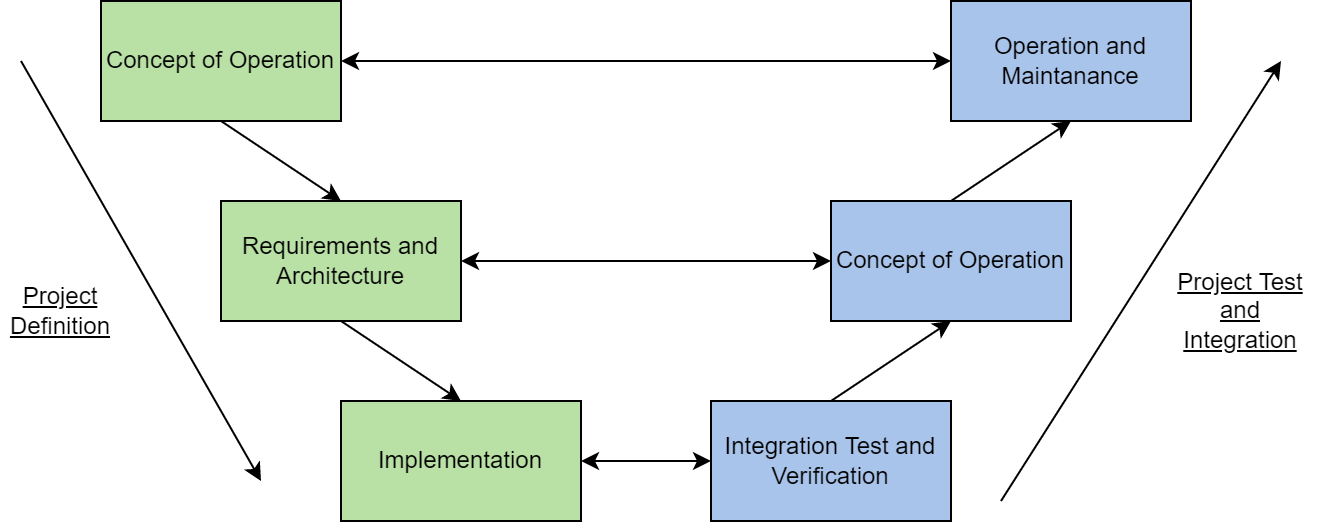
\includegraphics[width=\columnwidth]{V-Model.png}
    \caption{The V-Model helps in an IT-Project to have a focus on planning and implementation while reflecting and testing the program.}
    \label{fig:V-Model}
\end{figure}

Starting with the concept of operation stage. In this stage the plan is made and research is conducted. Second the requirements and architecture is decided. This covers the process of building a development system that is near to the production environment. In this project the production system is the NVIDIA Jetson and the development system the \acrlong{vm}. Splitting up the problem to find an optimum path into two smaller ones like the exploration and optimization algorithm helped to divide the workload and having the four eye principle on each other's code. The last part covers the implementation of the algorithms in the development environment and testing it. At the same time test definition on how to test the algorithms and how to verify a good one has to be done. The integration test and verification is covered in chapter \ref{ch:Results}. The concept of Operation process consists of the evaluation of the algorithms if they fit the criterion. Lastly the operation and maintenance phase deals with the integration of the algorithm into the production system. This is as well the combination of the exploration and optimization algorithm while using interfaces.

\subsection{Scrum} \label{sec:Planning Method: Scrum}
To ensure the communication between supervisors and developers Scrum was used. To get a deeper understanding how Scrum works an explanation in the appendix under \ref{sec:Scrum}. Weekly meetings where held with supervisors and biweekly meetings with the driverless team. In addition, the team itself held a meeting on a weekly basis as well. From the meeting notes user stories were created to translate the stories into code. Before the weekly meeting with the supervisors an e-mail is sent which covered the tasks that have been done in the past week, the task for the week after and problems the team faced during development.

\subsubsection{Kanban Board} \label{sec:Kanban Board}
The kanban board helps to organize the user stories and to prioritize the stories in the development process. In addition, another kanban board was made to write the thesis. As shown in figure \ref{fig:Kanban Board Path Planning} there are four columns. The ``To Do'' list with all the ideas and inputs from supervisors. The ``In progress'' list shows the current tasks and the ``Review in progress'' is for the other team member to review the code. Finally, the ``Done'' column illustrates the finished tasks.
\begin{figure}[H]
    \centering
    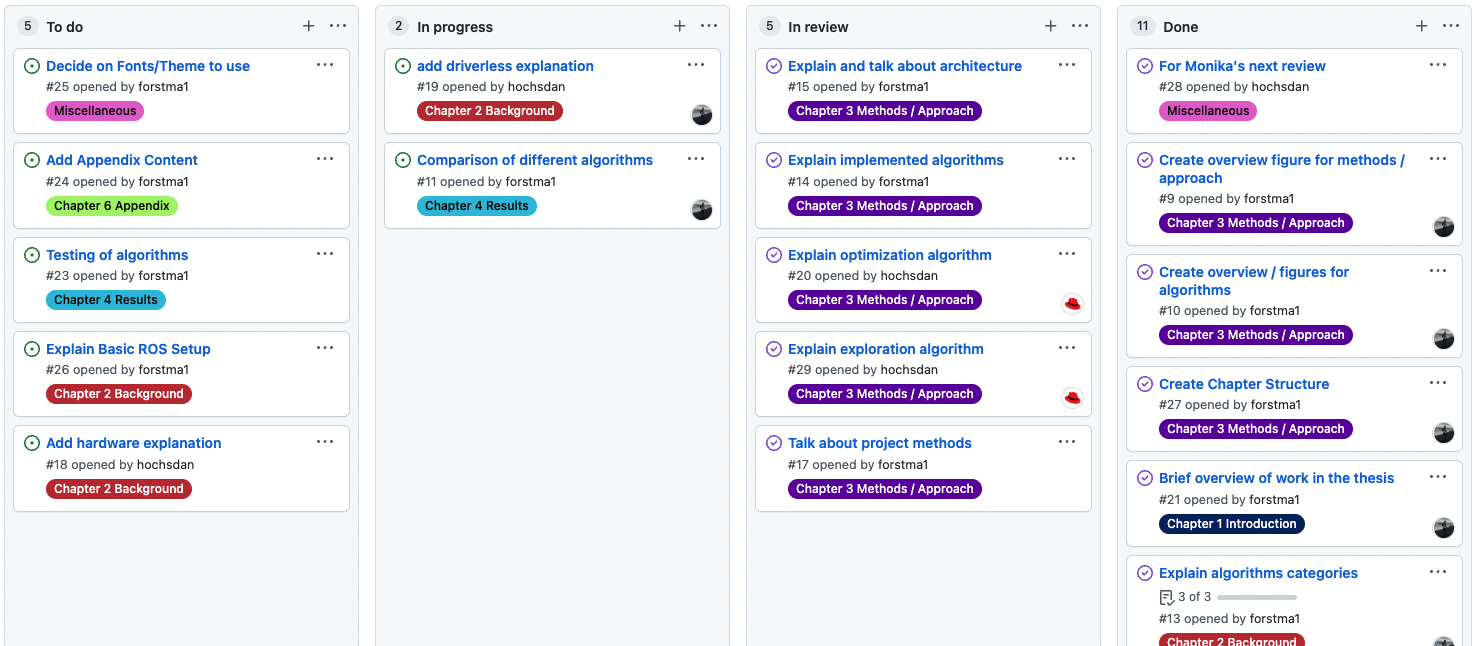
\includegraphics[width=\columnwidth]{Kanban_Board_Path_Planning.PNG}
    \caption{The Kanban Board helps to organize the user stories to see who is working on which story.}
    \label{fig:Kanban Board Path Planning}
\end{figure}


\section{Architecture Design} \label{sec:Architecture Design}
\begin{itemize}
    \item Beschreibt Architektur von ROS
    \item UML Klassendiagram
    \item Interfaces für Messages
    \item Kommunikationsdiagramm (zwischen Algorithmen)
\end{itemize}


\subsection{Development Environment} \label{sec:Development Environment}

\begin{itemize}
    \item ROS 2
    \item Python
    \item LaTeX
    \item Git
    \item VS Code
    \item Azure DevOps
    \item GitHub
    \item Simulation tools
    \item other tools
\end{itemize}


There are different methods to build a development environment. An easy way to get started is to build a relatively similar system like the one which is running on the NVIDIA Jetson computer. This computer will be used in the real car. A \acrlong{vm} (\acrshort{vm}) is a piece of software that can emulate hardware and encapsulates an operating system from the host operating system, that is running on hardware. Figure \ref{fig:Development Architecture} illustrates the architecture that is used for developing.

\begin{figure}[H]
    \centering
    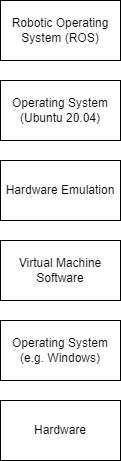
\includegraphics[width=2cm]{Development_Architecture.jpg}
    \caption{The development architecture consists of various levels: the hardware, the host operating system, the \acrlong{vm}, the operating system on the \acrshort{vm} and the \acrlong{ros}.}
    \label{fig:Development Architecture}
\end{figure}

On the NVIDIA Jetson computer an Ubuntu 20.04 operating system was installed. This is the reason why Ubuntu 20.04 is used on the development environment. An installation guide for how to install Ubuntu 20.04 in a \acrlong{vm} is found Cloud Linux Tech. \cite{cloudlinuxtech_install_ubuntu_2004}

\subsection{Robot Operating System (ROS)} \label{sec:Robot Operating System (ROS)}
The \acrlong{ros} (\acrshort{ros}) is not, like the name may suggest, a full-fledged operating system, but a set of software libraries and tools for the development of robot applications. The open-source robotics middleware comes shipped with capable developer tools, drivers and advanced algorithms. \cite{ros2_documentation}

There are currently two major versions of \acrshort{ros} which are seeing releases, ROS 1 and ROS 2. \cite{ros2_documentation} Beginning with releases after 'Foxy Fitzroy', releases in odd years will be non-LTS (Long Term Support) and will only be supported for 1.5 years, while new releases in even years are going to be long-term supported and will be supported for 5 years. \cite{ros2_documentation}

The work done in this thesis have been done using the ROS 2 release 'Foxy Fitzroy', released on June 5th, 2020. This release will be supported till the end of May 2023. \cite{ros2_releases_and_target_platforms}

\subsection{Integrated Development Environment (IDE) and Version Control} \label{sec:Integrated Development Environment (IDE) and Version Control}
For developing the \acrshort{ros} node an Integrated Development Environment (IDE) was used called Visual Studio Code. This IDE has the functionality to do syntax checking on the python and C++ code. Further on the IDE was used to write the thesis in Latex as an extension for building PDF files via Latex files can be installed. For both the code and the thesis a separate GIT Repository for version control was created. The version control system helps to develop in a software engineering team to follow changes on the code and in case of any problem it can be jumped back to an older code. The GIT server which was used is \href{https://github.zhaw.ch}{github.zhaw.ch}.

\section{Exploration Algorithm} \label{sec:Exploration Algorithm}
The exploration algorithm implementation is found in the python file: ``src/path\_planning/path\_planning/algorithm/exploration/exploration.py''. The algorithm uses several steps to get the middle line out of the cones position and car position on the track. Figure \ref{fig:Algorithm Exploration Figure A} and \ref{fig:Algorithm Exploration Figure B} are illustrating the different steps of the algorithm. Starting of with the steps (a) to (e) from figure \ref{fig:Algorithm Exploration Figure A}. The algorithm starts when more than 2 cones have been received from the ``cone\_publisher''. Step (a) shows 5 cones that have been received so far, the current position of the car and the next cone. After having enough cones the algorithm calculates the distance from the car to the newly received cone and evaluates the distance based on a threshold which is defined in a track configuration file. If the distance is in the threshold then new distances are calculated from the new cone to the previously received ones as shown in step (c). This distance has a different threshold and evaluates if the previously received cones are good for triangulation. Then the triangulation between the cones in the threshold and the new cone are calculated. This is shown in step (d). After the calculation of the triangles simplices are evaluated between the cones (e). These simplices or triangles consist of several edges.

\begin{figure}[H]
    \centering
    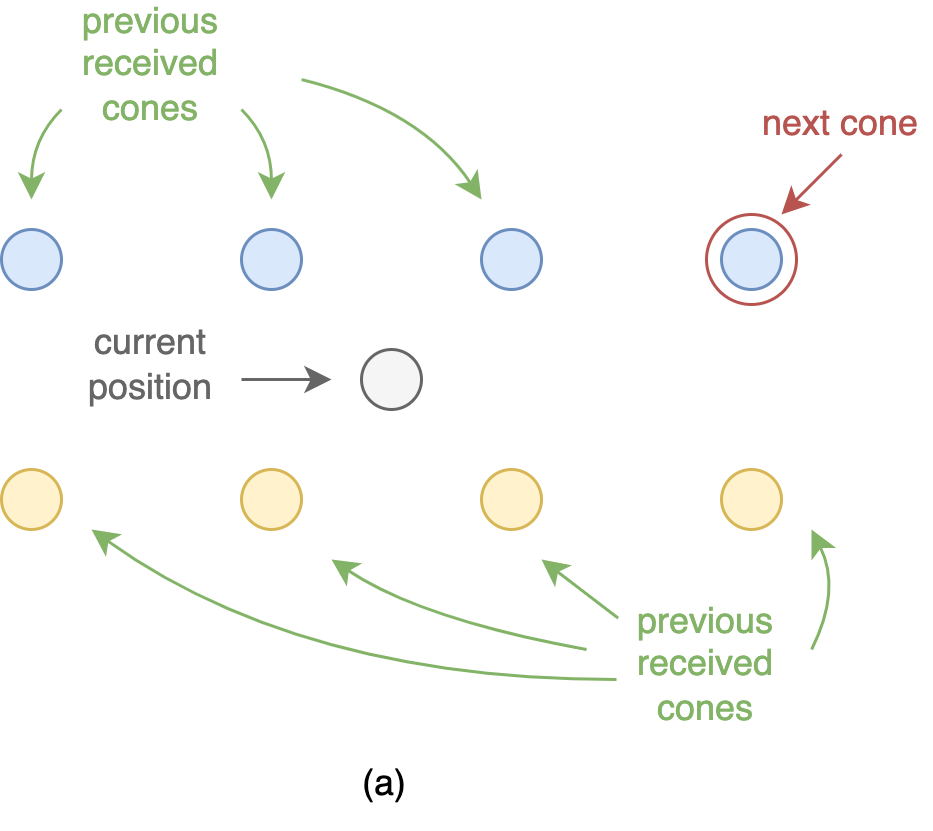
\includegraphics[width=5cm]{Algorithm_Exploration_Figure_A.png}
    \caption{The exploration algorithm covers the steps to find a middle line on the track. The first part of the algorithm describes the steps to find suitable cones for the triangulation algorithm (steps a to e).}
    \label{fig:Algorithm Exploration Figure A}
\end{figure}

Figure \ref{fig:Algorithm Exploration Figure B} shows the second part of the algorithm. It starts of based on the information of the edges between the new cones and cones in the given threshold. Step (f) shows how useful edges are validated. Edges which do not have the same tag meaning the same cone color on each side are not usable. The second criterion is that the edge can not be too long which becomes especially relevant in a curve on the track. This process of evaluation is repeated for every simplices (g). The next step (h) is to build a path. Since the path is not smooth an interpolation algorithm is used to straighten the path (i). After that the densify algorithm helps to have a path with more coordinates which is preciser (j). This path will then be published, and the optimization algorithm can use the generated points.

\begin{figure}[H]
    \centering
    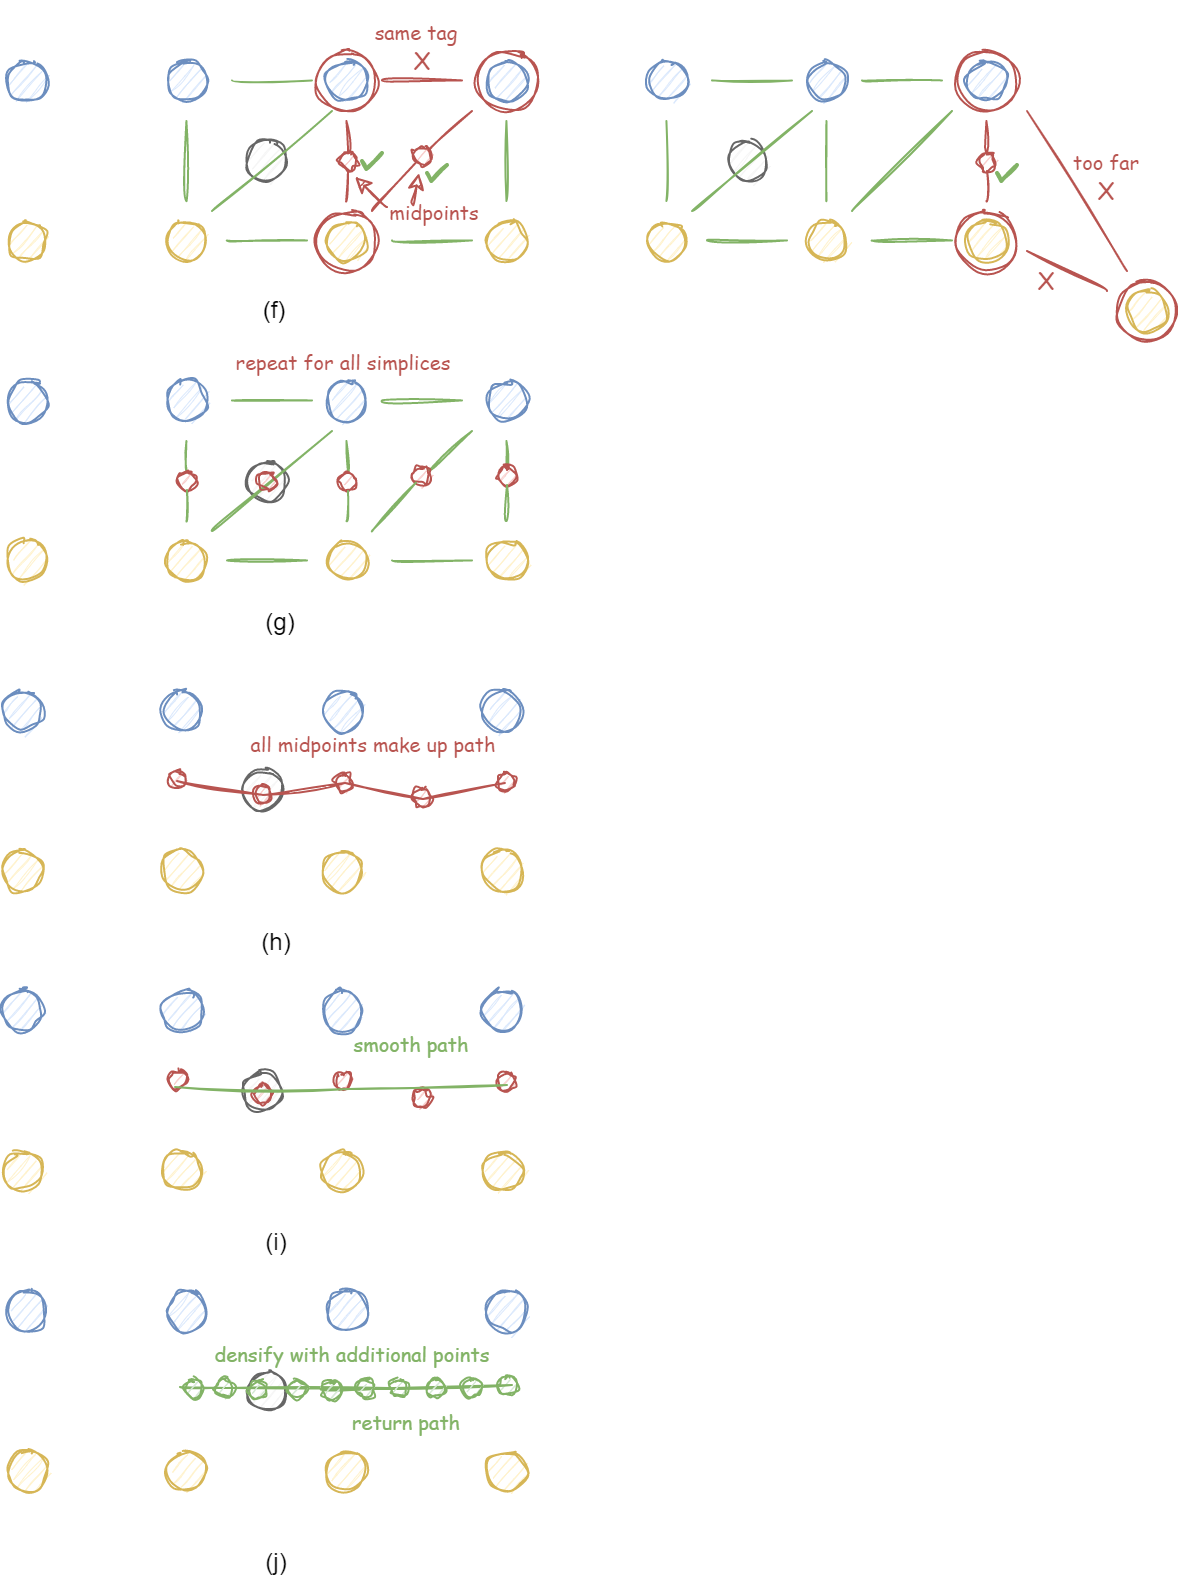
\includegraphics[width=6cm]{Algorithm_Exploration_Figure_B.png}
    \caption{The second part of the exploration algorithm covers criteria of suitable edges in a simplex, smoothening the path and denisifying the smoothed path.}
    \label{fig:Algorithm Exploration Figure B}
\end{figure}

Figure \ref{fig:Algorithm Exploration Pseudocode} shows the pseudocode of the exploration algorithm. Starting of with the distance from the current position of the car to the new cone the program checks if the distance is in the threshold. After that a list is created with all the past cones that are in a valid distance to the new cone. If the list is in the threshold of 3 or more cones than the triangulation is calculated. Further explanation is found in section \ref{sec:Motion Planning} under ``Combinatorial Motion Planning''. After the calculation of the simplices the edges were compared with each other so that no edges of the same ends are in the variable called ``edges''. After the comparison another loop is done to look if the cones on each edge do not have the same tag meaning the same color and are in a threshold. Each valid edge will be added to the ``pathOfMiddlepoints'' array. After the program knows the potential middle points a path smoothening algorithm is applied followed with a densify algorithm to add more middle points. The final result meaning the middle line as well as the track border is given to the optimization algorithm.

\begin{figure}[H]
    \centering
    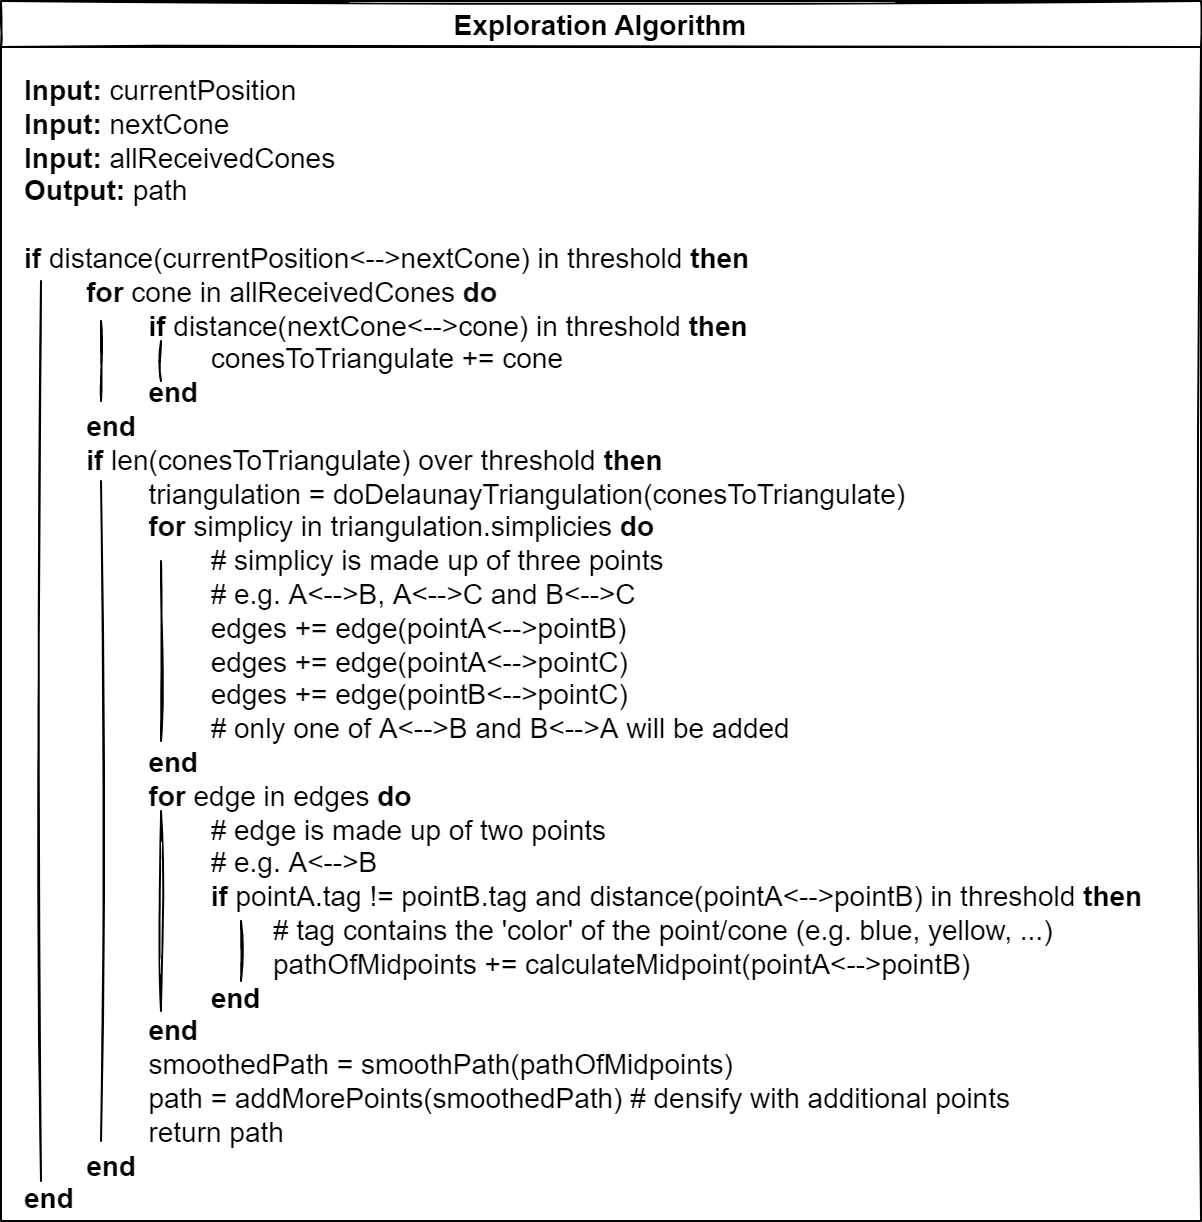
\includegraphics[width=6cm]{Algorithm_Exploration_Pseudocode.png}
    \caption{The exploration algorithm can be presented in a pseudocode program as well.}
    \label{fig:Algorithm Exploration Pseudocode}
\end{figure}

\section{Optimization Algorithm} \label{sec:Optimization Algorithm}
After the explore algorithm analyzed the middle line of the track the board computer switches to the optimization algorithm. For the base code of the algorithm we forked the code from \acrlong{tum} (\acrshort{tum}). \cite{tumftm_optimization_algoritm} 



\section{Integration and Verification} \label{sec:Integration and Verification}

\begin{itemize}
    \item Tests
    \item Integration (inkl. Switch)
    \item Verifikation über Simulationstool (wie ist das setup aufgebaut, welche strecken wurden getestet)
\end{itemize}

\subsection{Visual Test with Plots} \label{sec:Visual Test with Plots}
Several test methods have been used to integrate and validate the algorithms. The first method was the visual testing of plots. Python has a library called ``matplotlib.pyplot'' which can plot points, graphs and other structures on a coordinate system. To get an idea what a good algorithm is CSV files were used for getting the track information and publish it with the ``cone\_publisher'' node. The first step was to plot the full track with the start position of the car, the yellow and blue cones and the finish line which is represented with the orange cones. The second step was to test the exploration algorithm by plotting the triangulation. After that the middle points of the edges in the simplices where calculated and plotted on the coordinate system as well. This helped to get a feeling of what a good exploration algorithm looks like. The test results are found in chapter \ref{ch:Results}. Further on the path smoothening algorithm was tested visually in the coordinate system.

For the optimization algorithm a separate node was constructed which takes a CSV file with the middle line and the distance to the border of the track. Additionally, parameters of the physics of the car can be added to have an accurate perception of how fast the car should drive and what steering angle it should turn. The split of the logic of the algorithms was made to work separately on the code. The optimization algorithm has an output of the optimized track, an acceleration profile and steering angles on each point of the optimized path. The evaluation was done by plots. The same Python library was used to get an illustration of the result on a coordinate system.

\subsection{Integration} \label{sec:Integration}
The integration was done simultaneously since it is easy to integrate a python script into \acrshort{ros}. The first step is to define a type of node as described in section \ref{sec:ROS Nodes}. Then the python script has to be implemented via the ``import'' statement so that the class described in the algorithm Python script can be used in the \acrshort{ros} node. After that the node has to define a publisher statement which published the output of the algorithm. 

\subsection{Verification with the Simulation Tool} \label{sec:Verification with the Simulation Tool}


